\documentclass[a4paper,11pt] {article}
\usepackage[spanish]{babel}
\usepackage[utf8]{inputenc}
\usepackage{caratula}
\usepackage{a4wide}
\usepackage{graphicx}
% \usepackage{dot2texi}
% \usepackage{graphs}

\begin{document}

\titulo{Trabajo Pr\'actico}
\fecha{10/12/2009}
\materia{Sistemas Operativos}
\grupo{Nro. 10}
\integrante{Dinota, Mat\'ias}{076/07}{matiasgd@gmail.com}
\integrante{Leveroni, Luciano}{360/07}{lucianolev@gmail.com}
\integrante{Mosteiro, Agust\'in}{125/07}{agustinmosteiro@gmail.com}

\maketitle

\bigskip
\section*{Aclaraciones generales}

Antes de comenzar el an\'alisis de cada ejercicio, cabe mencionar lo siguiente: 

\section{Comandos básicos de Unix}

\begin{enumerate}
	\item \begin{enumerate}
		\item El directorio actual pasa a ser \textbf{/usr/bin}.
		\item El directorio actual pasa a ser \textbf{/home/tpsisop}.
		\item Al no ingresar ningún parámetro, el comando \textit{cd} cambia el directorio actual al directorio personal del usuario actual.
	\end{enumerate}
	\item El contenido del archivo es:
	\begin{verbatim}
# ~/.profile: executed by the command interpreter for login shells.
# This file is not read by bash(1), if ~/.bash_profile or ~/.bash_login
# exists.
# see /usr/share/doc/bash/examples/startup-files for examples.
# the files are located in the bash-doc package.

# the default umask is set in /etc/profile
#umask 022

# if running bash
if [ -n "$BASH_VERSION" ]; then
    # include .bashrc if it exists
    if [ -f "$HOME/.bashrc" ]; then
	. "$HOME/.bashrc"
    fi
fi

# set PATH so it includes user's private bin if it exists
if [ -d "$HOME/bin" ] ; then
    PATH="$HOME/bin:$PATH"
fi
	\end{verbatim}
	\item El único archivo encontrado es \textbf{/vmlinuz}.
	\item Se generó el directorio utilizando el comando \textbf{mkdir /home/tpsisop/tp}.
	\item Se copió el archivo utilizando el comando \textbf{cp /etc/passwd /home/tpsisop/tp/}.
	\item Se cambió el grupo utilizando el comando \textbf{chgrp tpsisop /home/tpsisop/tp/passwd}.
	\item Se cambió el usuario utilizando el comando \textbf{chown tpsisop /home/tpsisop/tp/passwd}.
	\item Se cambiaron los permiso del archivo \textbf{/home/tpsisop/tp/passwd}.
		\begin{itemize}
			\item Para que el propietario tenga permisos de lectura, escritura y ejecución: \textbf{chmod u$+$rwx /home/tpsisop/tp/passwd}.
			\item Para que el grupo tenga sólo permisos de lectura y ejecución: \textbf{chmod g$-$w$+$rx /home/tpsisop/tp/passwd}.
			\item Para que el resto tenga sólo permisos de ejecución: \textbf{chmod o$-$rw$+$x /home/tpsisop/tp/passwd}.
		\end{itemize}
	\item 
		\begin{itemize}
		 \item 	
			\begin{verbatim}
	 			127.0.0.1	localhost
			::1     ip6-localhost ip6-loopback
			\end{verbatim}
		 \item 	
		\end{itemize}
	\item La nueva password es \textit{guiguigui} con el comando \textbf{passwd}.
	\item Se borró el archivo con el comando \textbf{rm /home/tpsisop/tp/passwd}.
	\item Se enlazaron los archivos con los comandos \textbf{ln /etc/passwd /tmp/contra1}, \textbf{ln /etc/passwd /tmp/contra2} y \textbf{ln -s /etc/passwd /tmp/contra3} respectivamente.
	\item Se montó el CD-ROM de instalacion de Ubuntu JeOS con el comando \textbf{mount /dev/sr0/ /home/tpsisop/tp/}. El contenido del directorio es:
	\begin{verbatim}
		-r-xr-xr-x 1 root root   942 2008-04-22 03:07 cdromupgrade
		dr-xr-xr-x 3 root root  2048 2009-07-14 13:23 dists
		dr-xr-xr-x 3 root root  2048 2009-07-14 13:23 doc
		dr-xr-xr-x 3 root root  2048 2009-07-14 13:24 install
		dr-xr-xr-x 2 root root 12288 2009-07-14 13:24 isolinux
		-r--r--r-- 1 root root 47110 2009-07-14 13:24 md5sum.txt
		dr-xr-xr-x 2 root root  2048 2009-07-14 13:23 pics
		dr-xr-xr-x 4 root root  2048 2009-07-14 13:23 pool
		dr-xr-xr-x 2 root root  2048 2009-07-14 13:23 preseed
		-r--r--r-- 1 root root   228 2009-07-14 13:23 README.diskdefines
		lr-xr-xr-x 1 root root     1 2009-07-14 13:23 ubuntu -> .
	\end{verbatim}
	Se utilizó el comando \textbf{mount} para mostrar los siguientes \textit{filesystems} montados:
	\begin{verbatim}
		/dev/sda1 on / type ext3 (rw,relatime,errors=remount-ro)
		proc on /proc type proc (rw,noexec,nosuid,nodev)
		/sys on /sys type sysfs (rw,noexec,nosuid,nodev)
		varrun on /var/run type tmpfs (rw,noexec,nosuid,nodev,mode=0755)
		varlock on /var/lock type tmpfs (rw,noexec,nosuid,nodev,mode=1777)
		udev on /dev type tmpfs (rw,mode=0755)
		devshm on /dev/shm type tmpfs (rw)
		devpts on /dev/pts type devpts (rw,gid=5,mode=620)
		/dev/scd0 on /home/tpsisop/tp type iso9660 (ro)
	\end{verbatim}
	\item Se utilizó el comando \textbf{df} para mostrar el espacio libre de los \textit{filesystems} montados:
	\begin{verbatim}
		Filesystem            Size  Used Avail Use% Mounted on
		/dev/sda1             494M  423M   46M  91% /
		varrun                252M   32K  252M   1% /var/run
		varlock               252M     0  252M   0% /var/lock
		udev                  252M   40K  252M   1% /dev
		devshm                252M     0  252M   0% /dev/shm
		/dev/scd0             101M  101M     0 100% /home/tpsisop/tp
	\end{verbatim}
	\item TODO
	\item Se desmont\'o el CD-ROM de instalaci\'on de Ubuntu JeOS con el comando \textbf{unmount /dev/scd0}.
	\item La maquina virtual lleva 58 minutos de ejecuci\'on. Esto se corrobor\'o con el comando \textbf{uptime}.
	\item La versi\'on de kernel utilizada es la 2.6.24-24-virtual. Esta informaci\'on se obtuvo utilizando el comando \textbf{uname -a}.

\end{enumerate}

\section{Comandos Extendidos de Unix}

\begin{enumerate}
	\item Para escribir HOLA en la pantalla cada vez que se loguee un usuario se agreg\'o la siguiente l\'inea al archivo 	/etc/bash.bashrc:
	\textbf{echo "HOLA"}
	
	Para escribir BUENOS DIAS en la pantalla cada vez que se encienda la m\'aquina se agreg\'o la siguiente l\'inea al 			archivo /etc/rc.local:
	\textbf{echo "BUENOS DIAS"}
	
	Para escribir ADIOS en la pantalla cada vez que se desloguee un usuario se cre\'o un archivo llamado logout en el 			directorio /etc. El contenido del archivo es el siguiente:
	\textbf{echo "ADIOS"}
	Luego, se agreg\'o en el archivo /etc/rc.local la siguiente l\'inea:
	\textbf{trap '/etc/logout;exit' 0}
	
	Para escribir HASTA LA VISTA BABY en la pantalla cada vez que se apague la m\'aquina se agreg\'o la siguiente l\'inea 	al archivo /etc/rc0.d:
	\textbf{echo "HASTA LA VISTA BABY"}
	
	\item Para montar una imagen de floppy se utiliz\'o el siguiente comando:
		\textbf{mount -o loop imagen.img /media/floppy1/}
		
		Para montar una imagen iso se utiliz\'o el siguiente comando:
		\textbf{mount -o loop imagen.iso /media/iso/}
		
	\item Se agreg\'o un alias en el archivo .bashrc sin modificar su fecha (timestamp). Para esto se utiliz\'o el comando \textbf{touch -t timestamp}. El timestamp del archivo previo a la modificaci\'on se obtuvo con el comando  \textbf{ls -l}.
	El d\'ia y la hora del sistema se modific\'o con el comando \textbf{date timestamp}.
	
	\item TODO
	\item
		\begin{enumerate}
			\item Se guard\'o la informaci\'on en el archivo \textit{config} utilizando el comando \textbf{ls -Rl /etc > /home/tpsisop/tp/config}.
			\item El archivo \textit{config} posee 789 l\'ineas, 5061 palabras y 39070 caracteres. Se obtuvo la informaci\'on mediante el comando \textbf{wc config}.
			\item Se agrego el contenido ordenado del archivo \textit{/etc/passwd} al final del archivo \textit{config} con el comando \textbf{sort /etc/passwd $>>$ /home/tpsisop/tp/config}.
			\item El archivo \textit{config} posee 813 l\'ineas, 5090 palabras y 40051 caracteres. Se obtuvo la informaci\'on mediante el comando \textbf{wc config}.
			\item Se realiz\'o lo pedido ejecutando el siguiente comando: \textbf{ls -l /usr/bin/a* | grep apt | wc}.
		\end{enumerate}
	
\end{enumerate}

\section*{El kernel de Linux}
\subsection*{Funcionamiento del kernel linux}
	\begin{enumerate}
		\item Ej 1

		\item \textbf{Administraci\'on de la memoria}

		Para administrar la memoria linux utiliza un esquema de paginaci\'on por demanda de tres niveles con paginas fijas de 4KB. Dentro de este esquema cada proceso de usuario tiene su propio espacio de direcciones virtual. Mediante el uso de memoria swap se tiene un espacio virtual de 4GB donde 3 son para procesos de usuario y el restante para uso del kernel.
		
		Para administrar los tres niveles de paginaci\'on se utilizan las siguientes tablas:
			\begin{enumerate}
			\item Directorio global: cada proceso tiene solo una que ha de estar en memoria y su tamaño es de una p\'agina.
			\item Directorio intermedio de p\'aginas: puede ocupar varias p\'aginas. Cada entrada señala a una p\'agina de la tabla de p\'aginas final
			\item Tabla de p\'aginas: cada una de sus entradas hace referencia a la p\'agina virtual requerida.
			\end{enumerate}
		En cuanto a la administraci\'on de la memoria f\'isica, una parte es utilizada por el kernel. Esta partici\'on es permanente, es decir, ninguna de sus partes se pagina a disco.
		El resto de la memoria esta disponible para:
			\begin{enumerate}
			\item P\'aginas de usuario
			\item El cache de buffer: Contiene bloques de disco que se han leido recientemente, su tamaño es din\'amico y compite por la misma reserva de p\'aginas que las p\'aginas de usuario.
			\item El cache de paginaci\'on: formado por un conjunto de p\'aginas de usuario que ya no se necesitan y estan esperando que se les pagine a disco.
			\end{enumerate}

		\item 
			\begin{enumerate}
				\item \textbf{Sistema de archivos} 

				El sistema de archivos utilizado en UbuntuJeOS es extended 3 (ext3). Este sistema de archivos tiene un tipo de tabla de tamaño fijo donde se almacenan los i-nodos. Estos almacenan información del archivo como por ejemplo la ruta o path, tamaño, permisos, ubicación física, etc (la descripción completa de un i-nodo se presentará en posteriores secciones). En cuanto a la ubicación física, los i-nodos contienen referencias a bloques ubicados en el disco. Estos bloques son de tamaño especificable cuando se crea el sistema de archivos, desde los 512 bytes hasta los 4 KB, lo cual asegura un buen aprovechamiento del espacio libre con archivos pequeños.
	
				El espacio en ext3 está dividido en bloques, y los bloques organizados en grupos. Esto se hace para reducir la fragmentación externa y reducir al mínimo el número de búsquedas de disco cuando se lee una gran cantidad de datos consecutivos.
				Cada bloque contiene un superbloque grupo, el grupo de bloques de mapa de bits, mapa de bits i-nodo, seguidos por los bloques de datos reales.
				El superbloque contiene información importante que es crucial para el arranque del sistema operativo, con lo que las copias se realizan en cada bloque de grupo de cada bloque en el sistema de archivos. Sin embargo, sólo la primera copia de la misma, que se encuentra en el primer bloque del sistema de archivos, se utiliza en el arranque.
				El grupo descriptor almacena el valor del bloque de mapa de bits, mapa de bits inodo y el comienzo de la tabla de i-nodos por cada bloque de grupo y estos, a su vez, se almacena en un grupo descriptor tabla.
		
				A diferencia de su antecesor ext3 implementa un sistema de registro por diario (journaling) para hacer posible el uso de transacciones. Este sistema se basa en mantener un registro en el que se almacena la información necesaria para restablecer los datos afectados por la transacción en caso de que esta falle.

				\item El kernel de Linux contiene una capa llamada Virtual File System (VFS) que se utiliza en las system call que actúan sobre archivos. El VFS es una capa de indirección encargada de recibir las llamadas al sistema relacionadas al manejo de archivos y llamar a las funciones necesarias en el sistema de archivos físico. 
				Cuando un proceso hace una llamada al sistema para acceder a un archivo, el kernel llama a una función en el VFS. Esta función hace las operaciones que son independientes a la estructura del archivo y llama a la correspondiente función en el sistema de archivos físico para realizar las operaciones que dependen de la estructura. A continuación se presenta una figura que presenta el esquema mencionado.
				\begin{center}
				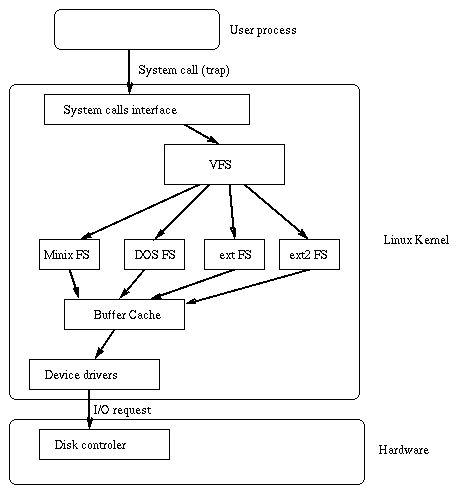
\includegraphics[width=0.65\textwidth]{ext2-vfs.png}
				\end{center}

			\end{enumerate}


		

		
	\end{enumerate}

\section*{Temas del Sistema Operativo}

\begin{enumerate}
  \item \textbf{Comunicaci\'on}
    Para realizar transferencia de archivos entre la m\'aquina virtual y el sistema operativo anfitri\'on se opt\'o por utilizar carpetas compartidas. Esto se logr\'o mediante los siguientes pasos:
    \begin{itemize}
      \item Dentro de la m\'aquina virtual se accede a \textit{Directorios compartidos} dentro del men\'u \textit{Dispositivos}.
      \item Se selecciona la carpeta que se desea compartir en la m\'aquina anfitrion y se le asigna un nombre.
      \item Se ejecuta el comando \textbf{mount -t vboxsf 'nombre-carpeta' $/$mnt$/$} para montar la carpeta compartida en la m\'aquina virtual.
    \end{itemize}

  \item \textbf{File System}
    Los \textit{hardlinks} apuntan a una estructura llamada i-nodo que contiene información sobre el archivo al que hace referencia el link y punteros a los bloques de memoria física en donde está alojado dicho archivo. Cada i-nodo almacena en uno de sus campos la cantidad de links que existen al archivo al que referencia. De este modo, sólo se elimina un i-nodo, y su correspondiente archivo, cuando la cantidad de links al archivo es 0, es decir, si se elimina un \textit{hardlink}, pero siguen existiendo links al archivo, este no será eliminado.
    Un i-nodo contiene la siguiente información:
    \begin{itemize}
      \item Modo (tipo de archivo y permisos)
      \item Cantidad de links
      \item UID del owner
      \item GID del owner
      \item Tamaño del archivo (en bytes)
      \item Fecha en la que el archivo fue accedido por última vez
      \item Fecha en la que el archivo fue modificado por última vez
      \item Fecha en la que el i-nodo fue modificado por última vez
      \item 12 punteros a bloques
      \item 1 puntero indirecto a bloques
      \item 1 puntero doble indirecto a bloques
      \item 1 puntero triple indirecto a bloques
      \item Estado del i-nodo (flags)
      \item Cantidad de bloques que ocupa el archivo
      \item Campos extra o reservados
    \end{itemize}

  \item \textbf{Prioridades}

    Para lograr ejecutar procesos con distintas prioridades utilizamos el comando \textbf{nice}. En este caso se quieren ejecutar tres procesos (\textit{loop1}, \textit{loop2} y \textit{loop3}) y darle mayor prioridad a uno de ellos. Con este objetivo se ejecutaron los procesos \textit{loop1} y \textit{loop2} asignandoles una muy baja prioridad (\textbf{nice -15 ./loop1} y \textbf{nice -15 ./loop2}). Luego se ejecut\'o el proceso \textit{loop3} normalmente logrando asi que tenga m\'as prioridad que los otros procesos mencionados.

    Para verificar el uso del CPU por parte de cada uno de los procesos se utiliz\'o el comando \textbf{top}. De esta manera se obtuvieron los siguientes resultados:
    \begin{itemize}
      \item \textit{loop1}: 3.3\%
      \item \textit{loop2}: 3.3\%
      \item \textit{loop3}: 93.1\%
    \end{itemize}

\end{enumerate}



\end{document}